\section{Experimental Results}\label{s:results}

\subsection{Histograms}\label{ss:results-histograms}


\begin{figure}[H]
\centering
\centerline{
\begin{minipage}{.5\linewidth}
  \centering
  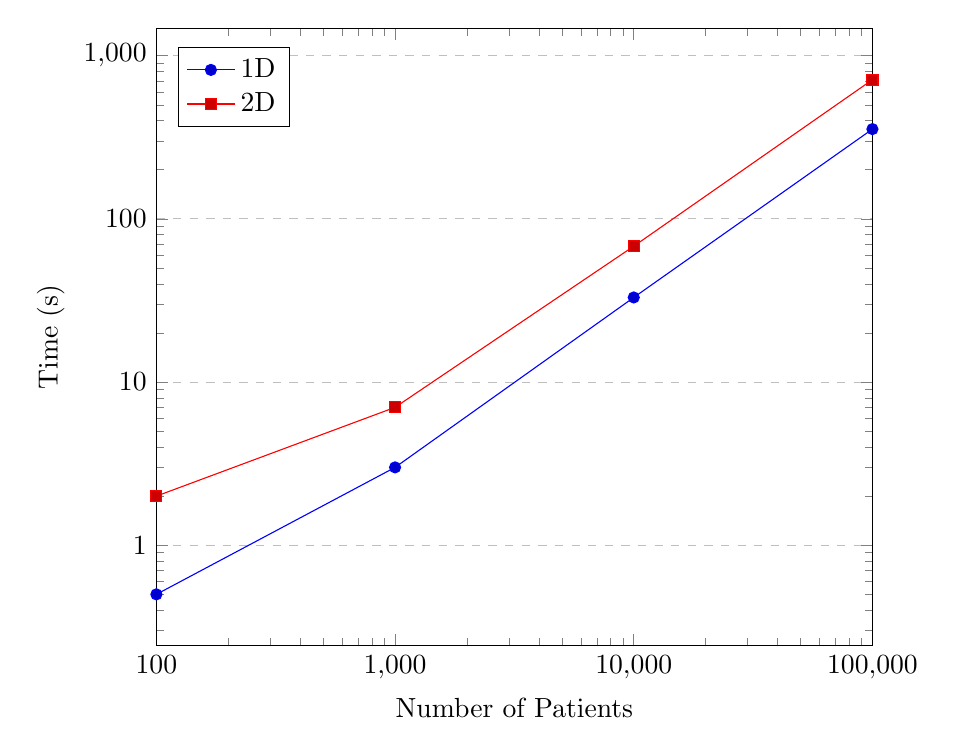
\begin{tikzpicture}
  \begin{axis}[
    legend pos=north west,
    scale only axis,
    enlarge x limits=-1,
    width=\textwidth*0.75,
    ymajorgrids=true,
    xmode=log,
    ymode=log,
    log ticks with fixed point,
    xlabel={Number of Patients},
    ylabel={Time (s)},
    ymin=0,
    grid style=dashed
  ]
  \addplot
    coordinates {(100, 0.5)(1000, 3)(10000, 33)(100000, 355)};
    \addlegendentry{1D}
  \addplot
    coordinates {(100, 2)(1000, 7)(10000, 68)(100000, 713)};
    \addlegendentry{2D}
  \end{axis}
  \end{tikzpicture}
  \caption{Numerical histograms timings}
\end{minipage}%
\begin{minipage}{.5\linewidth}
  \centering
  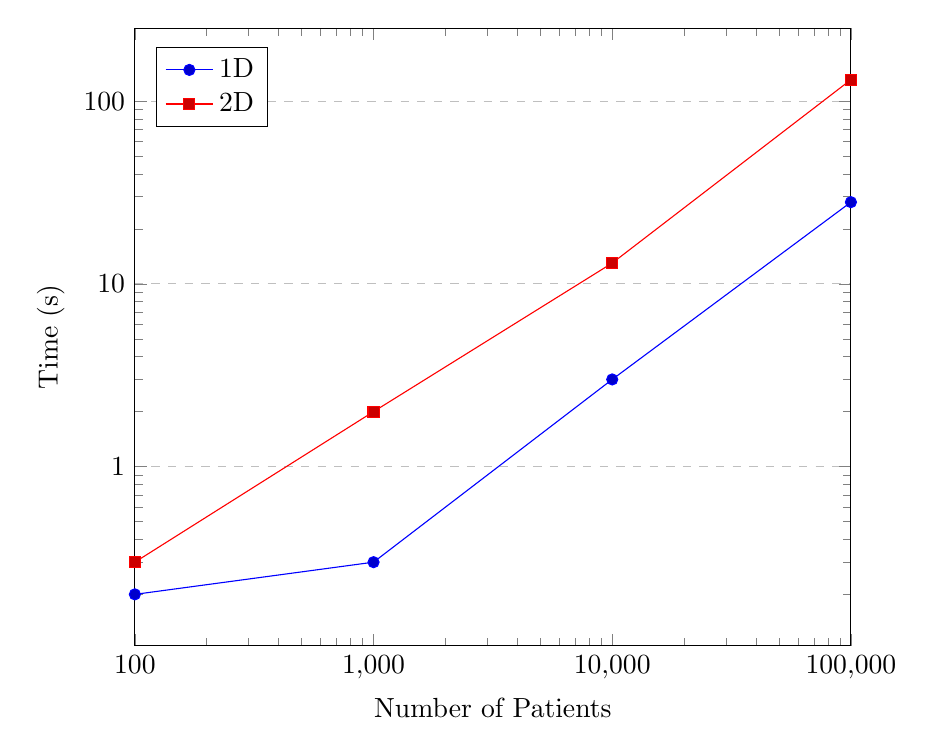
\begin{tikzpicture}
  \begin{axis}[
    legend pos=north west,
    scale only axis,
    enlarge x limits=-1,
    width=\textwidth*0.75,
    ymajorgrids=true,
    xmode=log,
    ymode=log,
    log ticks with fixed point,
    xlabel={Number of Patients},
    ylabel={Time (s)},
    ymin=0,
    grid style=dashed
  ]
  \addplot
    coordinates {(100, 0.2)(1000, 0.3)(10000, 3)(100000, 28)};
    \addlegendentry{1D}
  \addplot
    coordinates {(100, 0.3)(1000, 2)(10000, 13)(100000, 131)};
    \addlegendentry{2D}
  \end{axis}
  \end{tikzpicture}
  \caption{Categorical histograms timings}
\end{minipage}
}
\end{figure}


%%%%%%%%%%%%%%%%%%%%%%%%%%%%%%%%%%%%%%%%%%%%%%%%%%%%%%%%%%%%%%%%%%%%%%%%%%%%%%%%%%%

\begin{figure}[H]
\centering
\centerline{
\begin{minipage}{.8\linewidth}
  \centering
  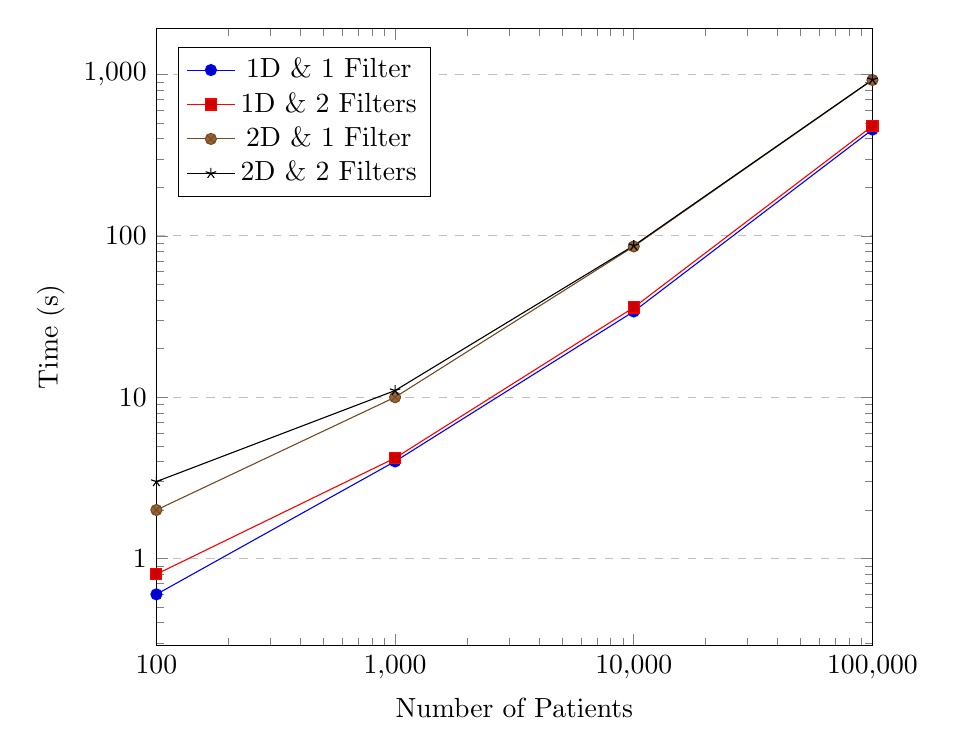
\begin{tikzpicture}
  \begin{axis}[
    legend pos=north west,
    scale only axis,
    enlarge x limits=-1,
    width=\textwidth*0.75,
    ymajorgrids=true,
    xmode=log,
    ymode=log,
    log ticks with fixed point,
    xlabel={Number of Patients},
    ylabel={Time (s)},
    ymin=0,
    grid style=dashed
  ]
  \addplot
    coordinates {(100, 0.6)(1000, 4)(10000, 34)(100000, 456)};
    \addlegendentry{1D \& 1 Filter}
  \addplot
    coordinates {(100, 0.8)(1000, 4.2)(10000, 36)(100000, 480)};
    \addlegendentry{1D \& 2 Filters}
  \addplot
    coordinates {(100, 2)(1000, 10)(10000, 86)(100000, 925)};
    \addlegendentry{2D \& 1 Filter}
  \addplot
    coordinates {(100, 3)(1000, 11)(10000, 87)(100000, 929)};
    \addlegendentry{2D \& 2 Filters}
  \end{axis}
  \end{tikzpicture}
  \caption{Numerical histograms with filters timings}
\end{minipage}%
}
\end{figure}


%%%%%%%%%%%%%%%%%%%%%%%%%%%%%%%%%%%%%%%%%%%%%%%%%%%%%%%%%%%%%%%%%%%%%%%%%%%%%%%%%%%
\begin{figure}[H]
\centering
\centerline{
\begin{minipage}{.8\linewidth}
  \centering
  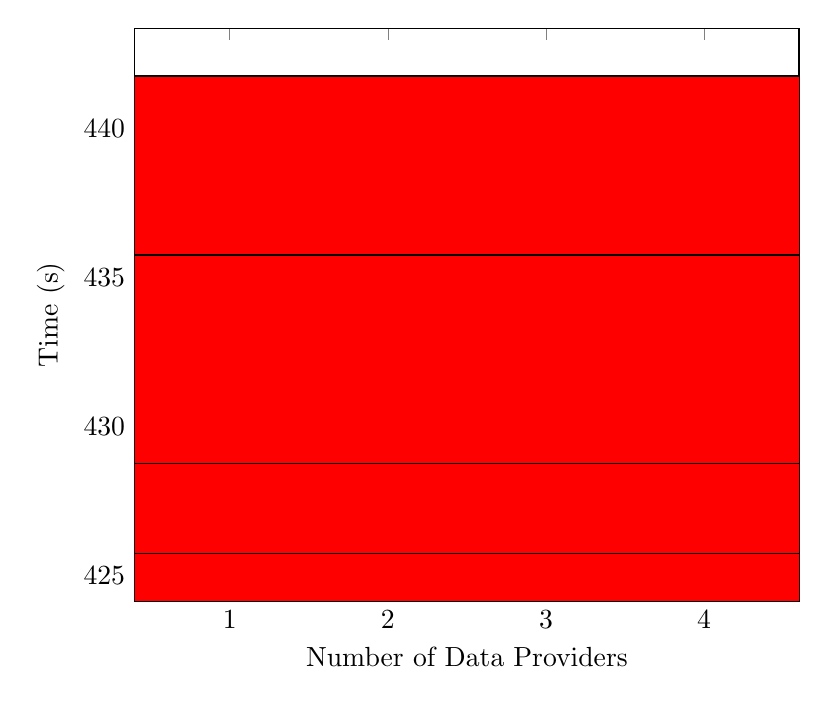
\begin{tikzpicture}
  \begin{axis}[
    legend pos=north west,
    scale only axis,
    ymajorgrids=true,
    xlabel={Number of Data Providers},
    ylabel={Time (s)},
    xtick = {1, 2, 3, 4},
    % ymin = 0,
    grid style=dashed,
    enlarge x limits = 0.2,
    bar width = 40
  ]
  \addplot[ybar, fill=red]
    coordinates {(1, 441.75)(2, 435.75)(3, 428.75)(4, 425.75)};
  \end{axis}
  \end{tikzpicture}
  \caption{Numerical histogram from variable data providers}
\end{minipage}%
}
\end{figure}


% \begin{figure}[H]
% \centering
% \centerline{
% \begin{minipage}{.5\linewidth}
%   \centering
%   \begin{tikzpicture}
%   \begin{axis}[
%     legend pos=north west,
%     scale only axis,
%     enlarge x limits=-1,
%     width=\textwidth*0.75,
%     ymajorgrids=true,
%     xmode=log,
%     ymode=log,
%     log ticks with fixed point,
%     xlabel={Number of Patients},
%     ylabel={Time (s)},
%     ymin=0,
%     grid style=dashed
%   ]
%   \addplot
%     coordinates {(100, 5.66)(1000, 10.54)(10000, 57.94)(100000, 536.09)};
%     \addlegendentry{1 data\hyp provider}
%   \addplot
%     coordinates {(100, 54.29)(1000, 56.5)(10000, 75.95)(100000, 267.7)};
%     \addlegendentry{2 data\hyp providers}
%   \addplot
%     coordinates {(100, 54.29)(1000, 56.5)(10000, 75.95)(100000, 267.7)};
%     \addlegendentry{3 data\hyp providers}
%   \end{axis}
%   \end{tikzpicture}
%   \caption{1-Dimensional numerical histograms timings for different number of data\hyp providers}
% \end{minipage}%
% \begin{minipage}{.5\linewidth}
%   \centering
%   \begin{tikzpicture}
%   \begin{axis}[
%     legend pos=north west,
%     scale only axis,
%     enlarge x limits=-1,
%     width=\textwidth*0.75,
%     ymajorgrids=true,
%     xmode=log,
%     ymode=log,
%     log ticks with fixed point,
%     xlabel={Number of Patients},
%     ylabel={Time (s)},
%     ymin=0,
%     grid style=dashed
%   ]
%   \addplot
%     coordinates {(100, 5.66)(1000, 10.54)(10000, 57.94)(100000, 536.09)};
%     \addlegendentry{1 data\hyp provider}
%   \addplot
%     coordinates {(100, 54.29)(1000, 56.5)(10000, 75.95)(100000, 267.7)};
%     \addlegendentry{2 data\hyp providers}
%   \addplot
%     coordinates {(100, 54.29)(1000, 56.5)(10000, 75.95)(100000, 267.7)};
%     \addlegendentry{3 data\hyp providers}
%   \end{axis}
%   \end{tikzpicture}
%   \caption{2-Dimensional categorical histograms timings for different number of data\hyp providers}
% \end{minipage}
% }
% \end{figure}



%%%%%%%%%%%%%%%%%%%%%%%%%%%%%%%%%%%%%%%%%%%%%%%%%%%%%%%%%%%%%%%%%%%%%%%%%%%%%%%%%%%
%%%%%%%%%%%%%%%%%%%%%%%%%%%%%%%%%%%%%%%%%%%%%%%%%%%%%%%%%%%%%%%%%%%%%%%%%%%%%%%%%%%
%%%%%%%%%%%%%%%%%%%%%%%%%%%%%%%%%%%%%%%%%%%%%%%%%%%%%%%%%%%%%%%%%%%%%%%%%%%%%%%%%%%

\subsection{Decision Trees}\label{ss:results-dtrees}

\begin{figure}[H]
\centering
\centerline{
\begin{minipage}{.8\linewidth}
  \centering
  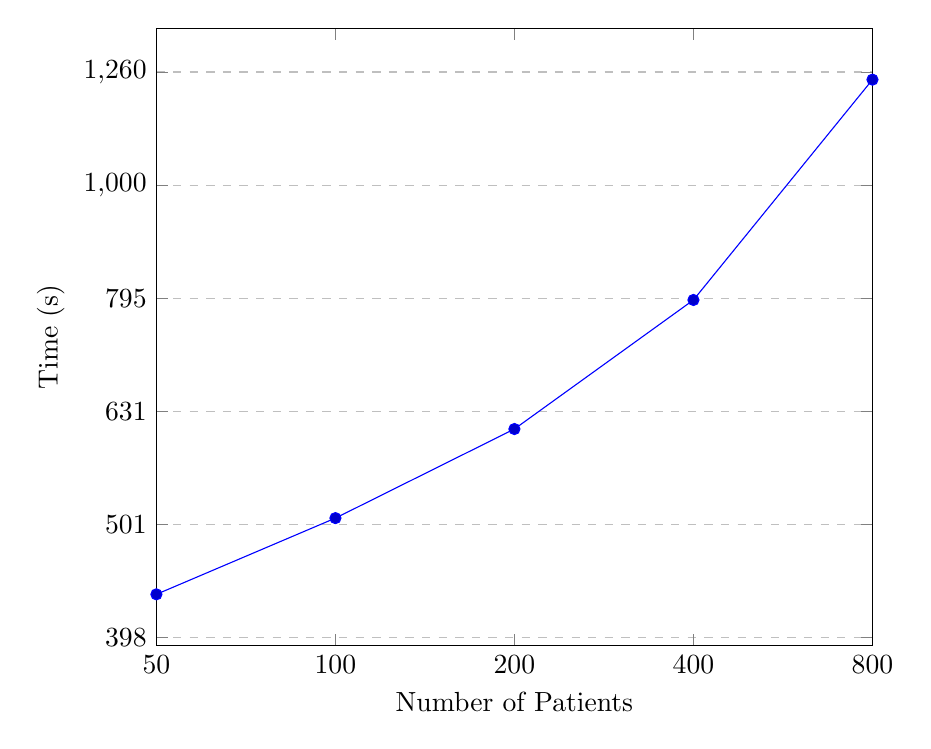
\begin{tikzpicture}
  \begin{axis}[
    legend pos=north west,
    scale only axis,
    enlarge x limits=-1,
    width=\textwidth*0.75,
    ymajorgrids=true,
    xmode=log,
    ymode=log,
    log ticks with fixed point,
    xlabel={Number of Patients},
    xtick = {50, 100, 200, 400, 800},
    ylabel={Time (s)},
    % ymin=0,
    log ticks with fixed point,
    grid style=dashed
  ]
  \addplot
    coordinates {(50, 435)(100, 508)(200, 609)(400, 792)(800, 1240)};
  \end{axis}
  \end{tikzpicture}
  \caption{ID3 decision tree classifier timings with variable patients}
\end{minipage}%
}
\end{figure}

\begin{figure}[H]
\centering
\centerline{
\begin{minipage}{.8\linewidth}
  \centering
  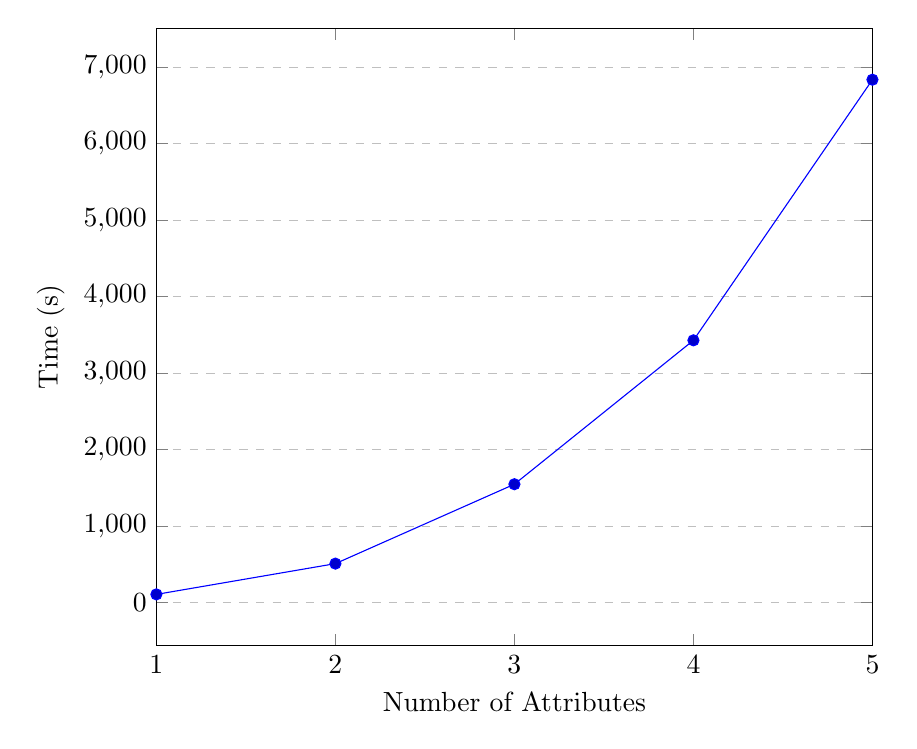
\begin{tikzpicture}
  \begin{axis}[
    legend pos=north west,
    scale only axis,
    enlarge x limits=-1,
    width=\textwidth*0.75,
    ymajorgrids=true,
    log ticks with fixed point,
    xlabel={Number of Attributes},
    xtick = {1, 2, 3, 4, 5},
    ylabel={Time (s)},
    % ymin=0,
    log ticks with fixed point,
    grid style=dashed
  ]
  \addplot
    coordinates {(1, 107)(2, 509)(3, 1547)(4, 3428)(5, 6835)};
  \end{axis}
  \end{tikzpicture}
  \caption{ID3 decision tree classifier timings with variable attributes}
\end{minipage}%
}
\end{figure}



%
%
% \begin{figure}[H]
% \centering
% \centerline{
% \begin{minipage}{.5\linewidth}
%   \centering
%   \begin{tikzpicture}
%   \begin{axis}[
%     legend pos=north west,
%     scale only axis,
%     enlarge x limits=-1,
%     width=\textwidth*0.75,
%     ymajorgrids=true,
%     xmode=log,
%     ymode=log,
%     log ticks with fixed point,
%     xlabel={Number of Patients},
%     ylabel={Time (s)},
%     ymin=0,
%     grid style=dashed
%   ]
%   \addplot
%     coordinates {(100, 0.548186)(1000, 5.381935)(10000, 52.661779)(100000, 530.589239)};
%     \addlegendentry{Num. ID3}
%   \addplot
%     coordinates {(100, 0.237847)(1000, 2.117192)(10000, 21.845599)(100000, 215.412621)};
%     \addlegendentry{Cat. ID3}
%   \addplot
%     coordinates {(100, 0.548186)(1000, 5.381935)(10000, 52.661779)(100000, 530.589239)};
%     \addlegendentry{Num. C4.5}
%   \addplot
%     coordinates {(100, 0.237847)(1000, 2.117192)(10000, 21.845599)(100000, 215.412621)};
%     \addlegendentry{Cat. C4.5}
%   \end{axis}
%   \end{tikzpicture}
%   \caption{ID3 \& C4.5 decision tree classifier timings for 3 attributes}
% \end{minipage}%
% \begin{minipage}{.5\linewidth}
%   \centering
%   \begin{tikzpicture}
%   \begin{axis}[
%     legend pos=north west,
%     scale only axis,
%     enlarge x limits=-1,
%     width=\textwidth*0.75,
%     ymajorgrids=true,
%     xmode=log,
%     ymode=log,
%     log ticks with fixed point,
%     xlabel={Number of Patients},
%     ylabel={Time (s)},
%     ymin=0,
%     grid style=dashed
%   ]
%   \addplot
%     coordinates {(100, 0.382224)(1000, 3.947421)(10000, 38.052168)(100000, 392.634467)};
%     \addlegendentry{Num. ID3}
%   \addplot
%     coordinates {(100, 0.099595)(1000, 0.922558)(10000, 9.712436)(100000, 99.149262)};
%     \addlegendentry{Cat. ID3}
%   \addplot
%     coordinates {(100, 0.382224)(1000, 3.947421)(10000, 38.052168)(100000, 392.634467)};
%     \addlegendentry{Num. C4.5}
%   \addplot
%     coordinates {(100, 0.099595)(1000, 0.922558)(10000, 9.712436)(100000, 99.149262)};
%     \addlegendentry{Cat. C4.5}
%   \end{axis}
%   \end{tikzpicture}
%   \caption{ID3 \& C4.5 decision tree classifier timings for 4 attributes}
% \end{minipage}
% }
% \end{figure}
%
%
% %%%%%%%%%%%%%%%%%%%%%%%%%%%%%%%%%%%%%%%%%%%%%%%%%%%%%%%%%%%%%%%%%%%%%%%%%%%%%%%%%%%
%
%
% \begin{figure}[H]
% \centering
% \centerline{
% \begin{minipage}{.5\linewidth}
%   \centering
%   \begin{tikzpicture}
%   \begin{axis}[
%     legend pos=north west,
%     scale only axis,
%     enlarge x limits=-1,
%     width=\textwidth*0.75,
%     ymajorgrids=true,
%     xmode=log,
%     ymode=log,
%     log ticks with fixed point,
%     xlabel={Number of Patients},
%     ylabel={Time (s)},
%     ymin=0,
%     grid style=dashed
%   ]
%   \addplot
%     coordinates {(100, 0.548186)(1000, 5.381935)(10000, 52.661779)(100000, 530.589239)};
%     \addlegendentry{1 data provider}
%   \addplot
%     coordinates {(100, 0.548186)(1000, 5.381935)(10000, 52.661779)(100000, 530.589239)};
%     \addlegendentry{2 data providers}
%   \addplot
%     coordinates {(100, 0.237847)(1000, 2.117192)(10000, 21.845599)(100000, 215.412621)};
%     \addlegendentry{3 data providers}
%   \end{axis}
%   \end{tikzpicture}
%   \caption{ID3 decision tree classifier timings for 3 attributes for different number of data\hyp providers}
% \end{minipage}%
% \begin{minipage}{.5\linewidth}
%   \centering
%   \begin{tikzpicture}
%   \begin{axis}[
%     legend pos=north west,
%     scale only axis,
%     enlarge x limits=-1,
%     width=\textwidth*0.75,
%     ymajorgrids=true,
%     xmode=log,
%     ymode=log,
%     log ticks with fixed point,
%     xlabel={Number of Patients},
%     ylabel={Time (s)},
%     ymin=0,
%     grid style=dashed
%   ]
%   \addplot
%     coordinates {(100, 0.548186)(1000, 5.381935)(10000, 52.661779)(100000, 530.589239)};
%     \addlegendentry{1 data provider}
%   \addplot
%     coordinates {(100, 0.548186)(1000, 5.381935)(10000, 52.661779)(100000, 530.589239)};
%     \addlegendentry{2 data providers}
%   \addplot
%     coordinates {(100, 0.237847)(1000, 2.117192)(10000, 21.845599)(100000, 215.412621)};
%     \addlegendentry{3 data providers}
%   \end{axis}
%   \end{tikzpicture}
%   \caption{C4.5 decision tree classifier timings for 3 attributes for different number of data\hyp providers}
% \end{minipage}
% }
% \end{figure}


